\documentclass{homework}
\usepackage[utf8]{inputenc}

\usepackage{graphicx}
\usepackage{float}
\graphicspath{ {./images/} }

\usepackage[fleqn]{amsmath}
\usepackage{amssymb}

\title{GPGN470A HW 5: Classification}
\author{Tyler Singleton}

\begin{document}
\maketitle

Question 1: \\ 

\begin{figure}[H]
    \centering
    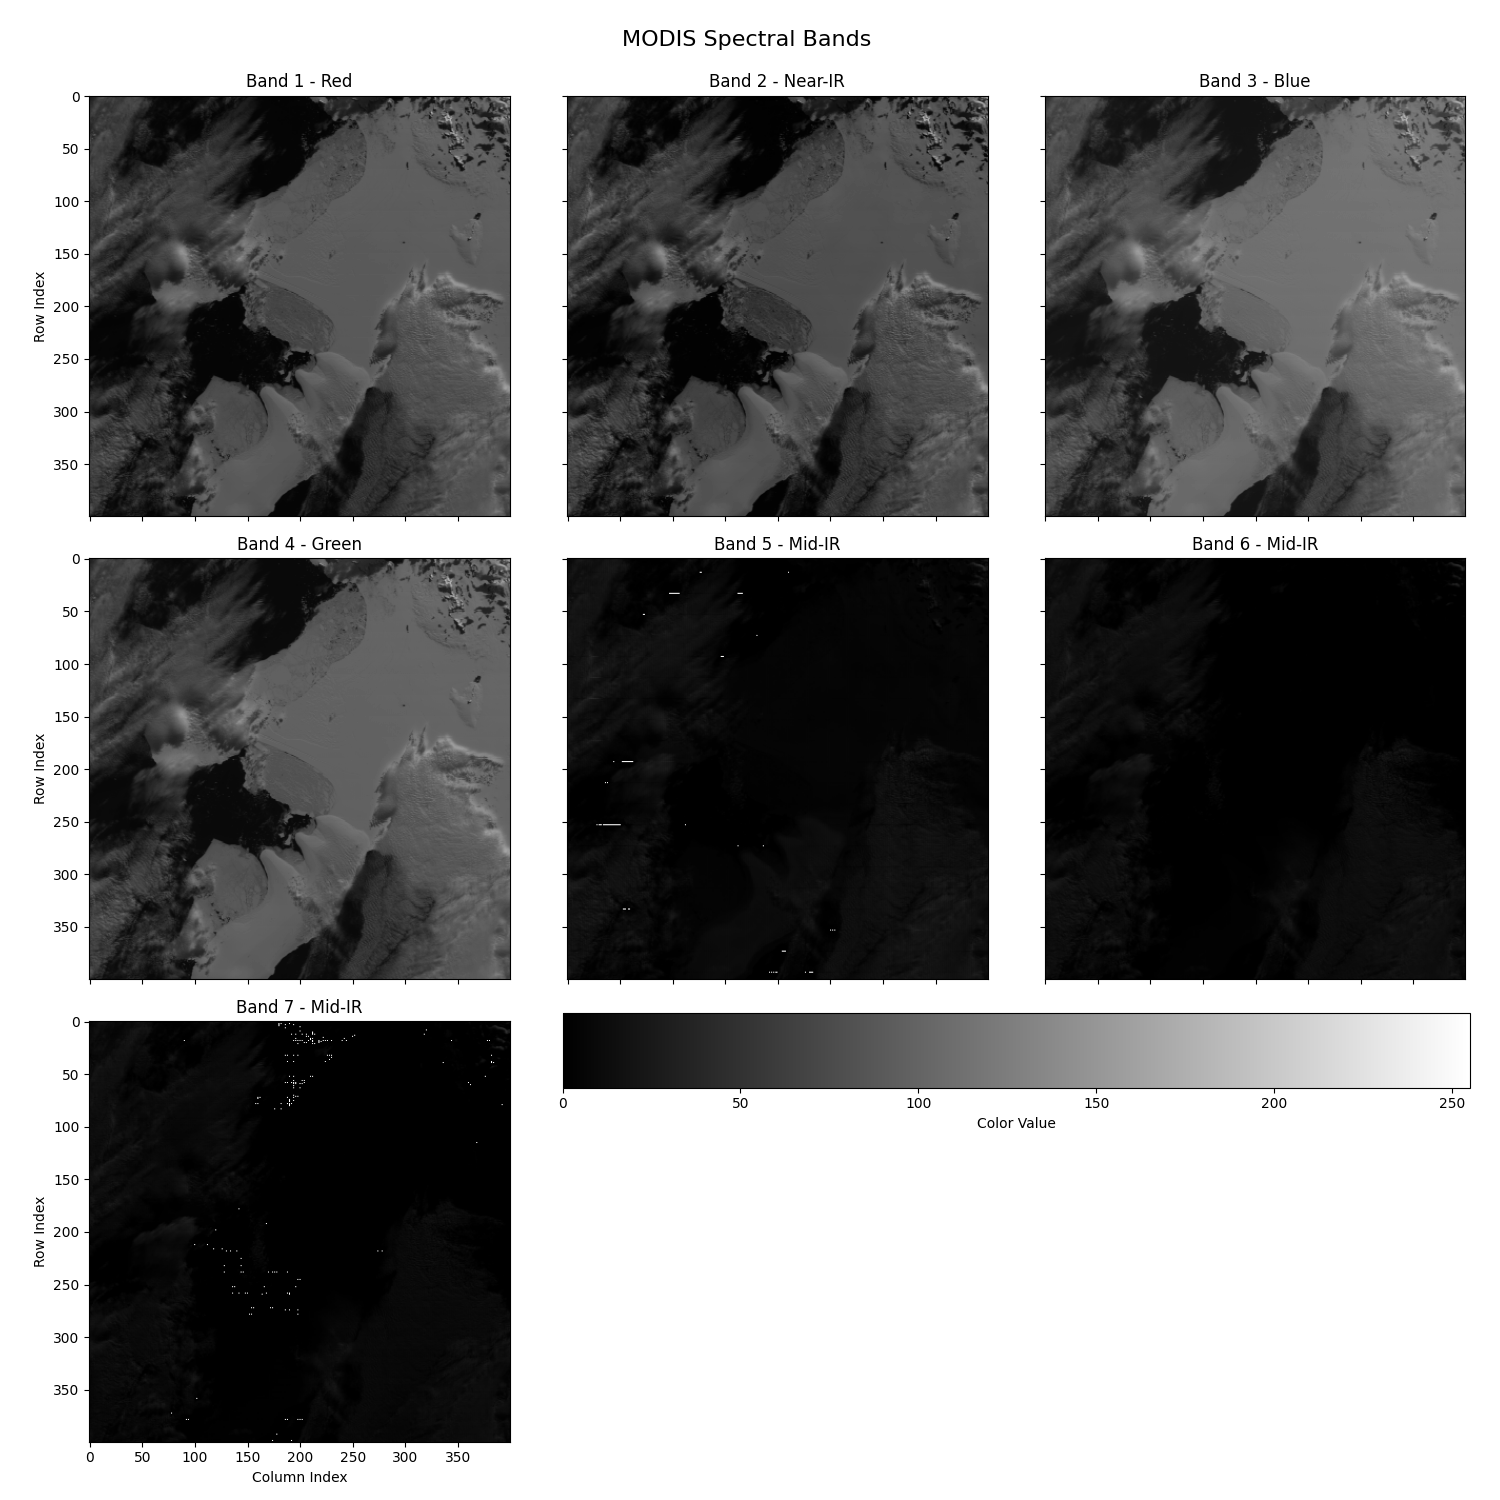
\includegraphics[width=\textwidth]{images/MODIS-GrayScale.png}
    \caption{Grayscale image from Bands 1-7.}
    \label{fig:GrayScale}
\end{figure}

\begin{figure}[H]
    \centering
    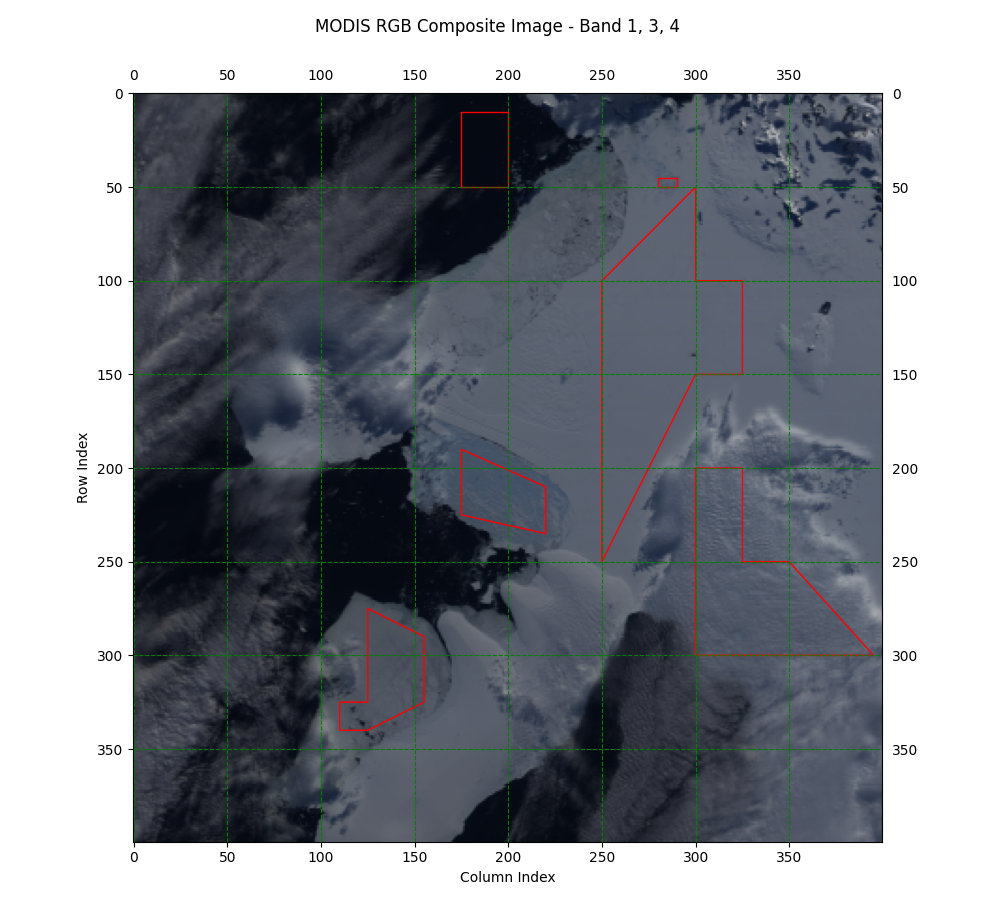
\includegraphics[width=\textwidth]{images/MODIS-RGB.png}
    \caption{RGB composite image using Bands 1, 3, and 4. Highlighted in red are the areas I used for my image classification algorithm.}
    \label{fig:RGB}
\end{figure}

%-----------------------------------------------%

Question 4: \\

\begin{figure}
    \centering
    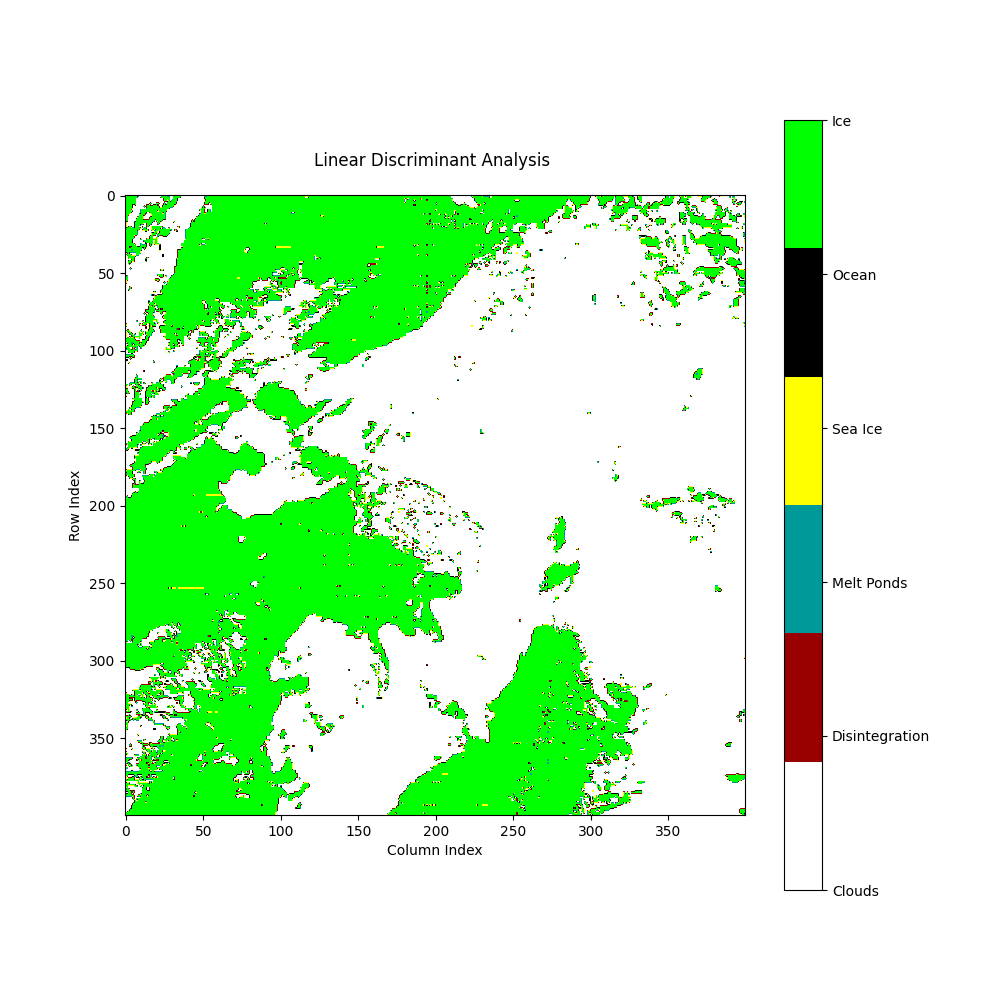
\includegraphics[width=\textwidth]{images/LinearDiscriminatAnalysis.png}
    \caption{The use of Linear Discriminant Analysis did not hold up well here. I believe my classes were too similar to each other that the algorithm blended most features together. The clouds appear to encompass both ice and land, while the ice is showing where the ocean should be. }
    \label{fig:Linear}
\end{figure}

\begin{figure}
    \centering
    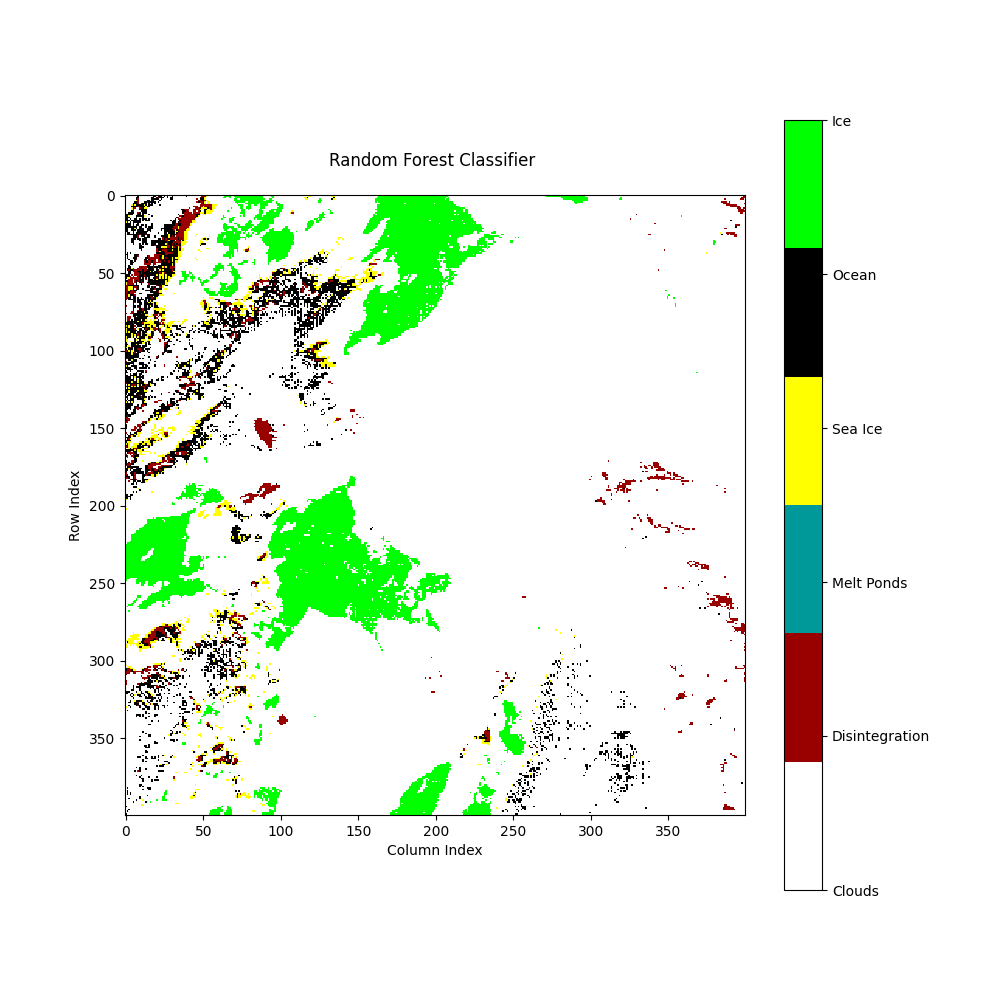
\includegraphics[width=\textwidth]{images/RandomForest.png}
    \caption{A random forest algorithm was used for this map with 100 estimators. This algorithm did a better job of distinguishing the ocean, but most classes were too similar for the algorithm to accurately categorize them separately.}
    \label{fig:Linear}
\end{figure}

\end{document}
